% arara: pdflatex: { synctex: yes }
% arara: makeindex: { style: ctuthesis }
% arara: bibtex

% The class takes all the key=value arguments that \ctusetup does,
% and a couple more: draft and oneside
\documentclass[oneside]{ctuthesis}
\usepackage{siunitx}
\usepackage{nomencl}
\usepackage{setspace}
\usepackage{indentfirst}

%%%%%%%%%%%%%%%%%% insert images from other directory
\usepackage{graphicx}
\graphicspath{{./images/}}

%%%%%%%%%%%%%%%%%%%%%%%%%%%%%%%%%%%%%% this shit is here to break long url into more lines
\usepackage{url}
\makeatletter
\g@addto@macro{\UrlBreaks}{\UrlOrds}
%\makeatother

%%%%%%%%%%%%%%%%%%%%%%%%%%%%%%%%%%%%%% this shit is here to prevent breaking words on the edge of a line
\tolerance=1
\emergencystretch=\maxdimen
\hyphenpenalty=10000
\hbadness=10000


% to print code
\usepackage{listings}
\usepackage{color}
\definecolor{dkgreen}{rgb}{0,0.6,0}
\definecolor{gray}{rgb}{0.5,0.5,0.5}
\definecolor{mauve}{rgb}{0.58,0,0.82}
\lstset{frame=tb,
  language=Java,
  aboveskip=3mm,
  belowskip=3mm,
  showstringspaces=false,
  columns=flexible,
  basicstyle={\small\ttfamily},
  numbers=none, 
  % numberstyle=\tiny\color{gray},
  % keywordstyle=\color{blue},
  % commentstyle=\color{dkgreen},
  % stringstyle=\color{mauve},
  breaklines=true,
  breakatwhitespace=true,
  tabsize=3
}
% to display source code
\definecolor{mGreen}{rgb}{0,0.6,0}
\definecolor{mGray}{rgb}{0.5,0.5,0.5}
\definecolor{mPurple}{rgb}{0.58,0,0.82}
\definecolor{backgroundColour}{rgb}{0.95,0.95,0.92}
\lstdefinestyle{CStyle}{
    backgroundcolor=\color{backgroundColour},   
    commentstyle=\color{mGreen},
    keywordstyle=\color{magenta},
    numberstyle=\tiny\color{mGray},
    stringstyle=\color{mPurple},
    basicstyle=\footnotesize,
    breakatwhitespace=false,         
    breaklines=true,                 
    captionpos=b,                    
    keepspaces=true,                 
    numbers=left,                    
    numbersep=5pt,                  
    showspaces=false,                
    showstringspaces=false,
    showtabs=false,                  
    tabsize=2,
    language=C
}


%%%
% \usepackage{framed}
% \usepackage{hyperref}
% % \usepackage[czech]{babel}
% \usepackage[utf8]{inputenc}
% \usepackage[T1]{fontenc}

\usepackage{dirtree}        %directory tree visualisation
\usepackage{blindtext}
\parskip=12pt % adds vertical space between paragraphs

\usepackage{xcolor}
\definecolor{shadecolor}{RGB}{230,230,230}

% to print code
\usepackage{listings}
\usepackage{color}
%%%

\ctusetup{
%	preprint = \ctuverlog,```%%%%%%%%%%%%%%%%%%%%%%%%% toto je cislo na kazde strance dole ktere tam nema byt
%	mainlanguage = english,
%	titlelanguage = english,
	mainlanguage = czech,
	otherlanguages = {czech},
	title-czech = {Low power wireless sensor network},
	title-english = {Low power wireless sensor network},
	subtitle-czech = {},
	subtitle-english = {},
	faculty = F3,
	department-czech = {Katedra telekomunikační techniky},
	department-english = {Department of Telecommunications Engineering},
	author = {Tomáš Hyhlík},
	supervisor = {Ing. Bc. Marek Neruda, Ph.D},
	supervisor-address = {},
	supervisor-specialist = {Ing. Bc. Lukáš Vojtěch, Ph.D},
	fieldofstudy-english = {Electronics and Communications},
	subfieldofstudy-english = {Electronics},
	fieldofstudy-czech = {Elektronika a komunikace},
	subfieldofstudy-czech = {Elektronika},
	% keywords-czech = {sensor network},
	% keywords-english = {sensor network},
	day = 12,
	month = 10,
	year = 2019,
	specification-file = {zav_prace.pdf},
%	front-specification = true,
%	front-list-of-figures = false,
%	front-list-of-tables = false,
%	monochrome = true,
%	layout-short = true,
}

\ctuprocess

\addto\ctucaptionsczech{%
	\def\supervisorname{Vedoucí}%
	\def\subfieldofstudyname{Studijní program}%
}

\ctutemplateset{maketitle twocolumn default}{
	\begin{twocolumnfrontmatterpage}
		% \ctutemplate{twocolumn.thanks}
		% \ctutemplate{twocolumn.declaration}
		\ctutemplate{twocolumn.abstract.in.titlelanguage}
		\ctutemplate{twocolumn.abstract.in.secondlanguage}	
		\ctutemplate{twocolumn.tableofcontents}
		\ctutemplate{twocolumn.listoffigures}
	\end{twocolumnfrontmatterpage}
}

% Theorem declarations, this is the reasonable default, anybody can do what they wish.
% If you prefer theorems in italics rather than slanted, use \theoremstyle{plainit}
\theoremstyle{plain}
\newtheorem{theorem}{Theorem}[chapter]
\newtheorem{corollary}[theorem]{Corollary}
\newtheorem{lemma}[theorem]{Lemma}
\newtheorem{proposition}[theorem]{Proposition}

\theoremstyle{definition}
\newtheorem{definition}[theorem]{Definition}
\newtheorem{example}[theorem]{Example}
\newtheorem{conjecture}[theorem]{Conjecture}

\theoremstyle{note}
\newtheorem*{remark*}{Remark}
\newtheorem{remark}[theorem]{Remark}

\setlength{\parskip}{5ex plus 0.2ex minus 0.2ex}

% % Abstract in Czech
% \begin{abstract-czech}
% Účelem této práce je...

% \end{abstract-czech}

% % Abstract in English
% \begin{abstract-english}
% The purpose of this work is...
% \end{abstract-english}

% % Acknowledgements / Podekovani
% \begin{thanks}
% I would like to thank Supervisor Ing. Bc. Marek Neruda Ph.D and Supervisor-specialist Ing. Bc. Lukáš Vojtěch Ph.D for helping me with this project. Also I would like to thank IMA s.r.o. company, which helped me to get compatible cards to the HID Prox Point plus reader, which is used for the second system design.
% \end{thanks}


% % Declaration / Prohlaseni
% \begin{declaration}
% I declare that I have developed the presented work independently and that I have
% listed all information sources used in accordance with the Methodical Guidelines on
% Maintaining Ethical Principles During the Preparation of Higher Education Theses.

% In Prague, \ctufield{day}.~\monthinlanguage{title}~\ctufield{year}
% \end{declaration}

% Only for testing purposes
\listfiles
\usepackage[pagewise]{lineno}
\usepackage{lipsum,blindtext}
\usepackage{mathrsfs} % provides \mathscr used in the ridiculous examples

\newcommand{\abbrlabel}[1]{\makebox[3cm][l]{\textbf{#1}\ \dotfill}}
\newenvironment{abbreviations}{\begin{list}{}{\renewcommand{\makelabel}{\abbrlabel}}}{\end{list}}


%%%%%%%%%%%%%%%%%%%%%%%%%%%%%%%%%  BEGIN %%%%%%%%%%%%%%%%%%%%%%%%%%%%%%%%%%%%%%%%%
\begin{document}

\maketitle

% \ctutemplate{specification.as.chapter}       % ZADANI

%\rule{\linewidth}{1pt}     % this shit was here for the url cut
\titlespacing*{\chapter}					{0pt}	{0ex}{0ex}
\titlespacing*{\section} 					{0pt}	{0ex}{-3ex}
\titlespacing*{\subsection} 			{0pt}	{0ex}{-3ex}
\titlespacing*{\subsubsection}		 {0pt}	{0ex}{-4ex}
\titlespacing*{\paragraph} 			{0pt}	{0ex}{-4ex}
\titlespacing*{\aubparagraph} 		{0pt}	{0ex}{-4ex}

% \section{List of Abbreviations}
\section{Seznam zkratek}
\begin{abbreviations}
	\item[AppSKey]	Application Session Key
	\item[CPU]		Central Processing Unit
	\item[CR] 			Carriage Return
	\item[CRC] 			Cyclic Redundancy Check
	\item[IoT] 		Internet of Things
	\item[LAN]		Local Area Network
	\item[LF]		Line Feed 
	\item[LPWAN]   	Low Power Wide Area Network 
	\item[LPWSN] 	Low Power Wireless Sensor Network	
	\item[MCU] 		Micro Controller Unit
	\item[NwkSKey]	Network Session Key
	\item[RF]		Radio Frequency
	% \item[BLE]   	Bluetooth Low Energy
	% \item[I2C]   	Inter-integrated Circuit
	% \item[IoT]		Internet of Things
	% \item[IPv6] 	Internet Protocol version 6
	% \item[ISM]		Industrial, scientific and medical

	% \item[M2M]		machine to machine
	% \item[RF]		Radio Frequency
	% \item[RPMA]		Random Phase Multiple Access
	% \item[SDK]	 	Software development kit
	\item[SF]		Spreading Factor
	% \item[SPI]   	Serial Peripheral Interface 
\end{abbreviations}


% \chapter{Introduction}
This chapter presents background, purpose and objectives to make clear the goal of this thesis.


\section{Background}
RFID technology is happening to be very popular these days for various applications such as industrial automation, access control, animal identification, public transport, event ticketing, parking, electronic wallet, goods identification and many more.
The question is how secure this technology is. The answer is, that there are various manufacturers providing RFID (Radio Frequency Identification) devices with various security. Information delivered by the manufacturers about the security should be clear.


\section{Why electronic door lock?}
However, there are very secure door locks, commonly used mechanical door lock has a lot of disadvantages. It's easy to clone keys and it's even possible to open the door without the key. If a key is lost, changing the lock is needed, which could be even impossible in some cases. Somebody who finds the lost key would be able to open the door.
Electronic door lock  might came out with solutions of these problems, however every lock is possible to hack somehow. 
A key of electronic door lock is usually RFID tag or card, but it can be also mobile phone communicating via bluetooth interface etc.
The user's card may be also used in other applications, like electronic purse.
In case that user loses his card, the card can be deleted from the system.
There is also so many advantages like user info can be stored on the RFID card and part of the system might be a server where scanned cards are monitored. 


\section{Objectives}
The purpose of this thesis is to design and assembly an RFID based access control system composed of inexpensive RFID devices used today and examine its security and possibility of hacking it. 
In the conclusions, it's assessed if the information given by the manufacturer gives a clear picture of the security of
his RFID technology.















		

% \part{Theoretical part}
													
% \chapter{Low power wireless network technologies}
In the appendix is table where all widely used low power wireless technologies are compared.
This chapter additionally provide a brief description of all these technologies, but the main parameters are only in the table.
All these technologies use license-free ISM bands.


\section{IQRF}
This technology aims to make it easy to implement wireless solutions. It enables peer-to-peer, star and mesh network communication modes. The IQRF alliance provide IQRF transceivers for \$15-20 with a few serial interfaces such as SPI, I2C, UART etc. and they also provide open source SDK which makes it very easy to use IQRF modules. The SDK is based on Java so it's compatible with various platforms such as Linux and Windows
\cite{1} \cite{2} \cite{3} \cite{4}.


\section{Wireless M-bus}
\textit{"Wireless Meter Bus has its origins within the Meter-Bus standards. This is a field bus standard aimed at applications for collecting meter data for gas, electricity, water, etc."} \cite{5}
It supports a few application modes for differing applications.
\begin{itemize}
  \item S1  Unidirectional, data are transmitted only a several times a day.
  \item S2	Bidirectional version of S1.
  \item	T1	Unidirectional transmission of data with a period of a few seconds of minutes.
  \item T2	Bidirectional version of T1.
  \item C1	Unidirectional transmission of bigger amount of data.
  \item C2	Bidirectional version of C1.
\end{itemize}
Usually one M-bus device support only a few of these application modes \cite{5} \cite{6} \cite{7} \cite{8}.


\section{Zigbee}
Zigbee, developed by zigbee alliance is usually used for mesh sensor networks because of its short range. This technology is standardized since 2003, so there is many available nodes at the market by now \cite{10} \cite{11} \cite{12}.

\section{Bluetooth}
Bluetooth has the big advantage, taht it's built in almost every mobile phone, tablet or laptop so there are more options to control the network. The Bluetooth 4.0+ also called BLE (Bluetooth Low Energy) aims to low power wireless sensor networks.
It can be used for point-to-point, broadcast or mesh network topology \cite{13} \cite{14} \cite{15} \cite{16}.


\section{LoRa}
The name LoRa stands for "Long Range" wireless communication with low data rate and power consumption. The protocol enables to modify SF which affects the communication range and data rate. The \ref{fig:loraSF} shows this dependence.

\begin{figure}[!h]
    \centering
    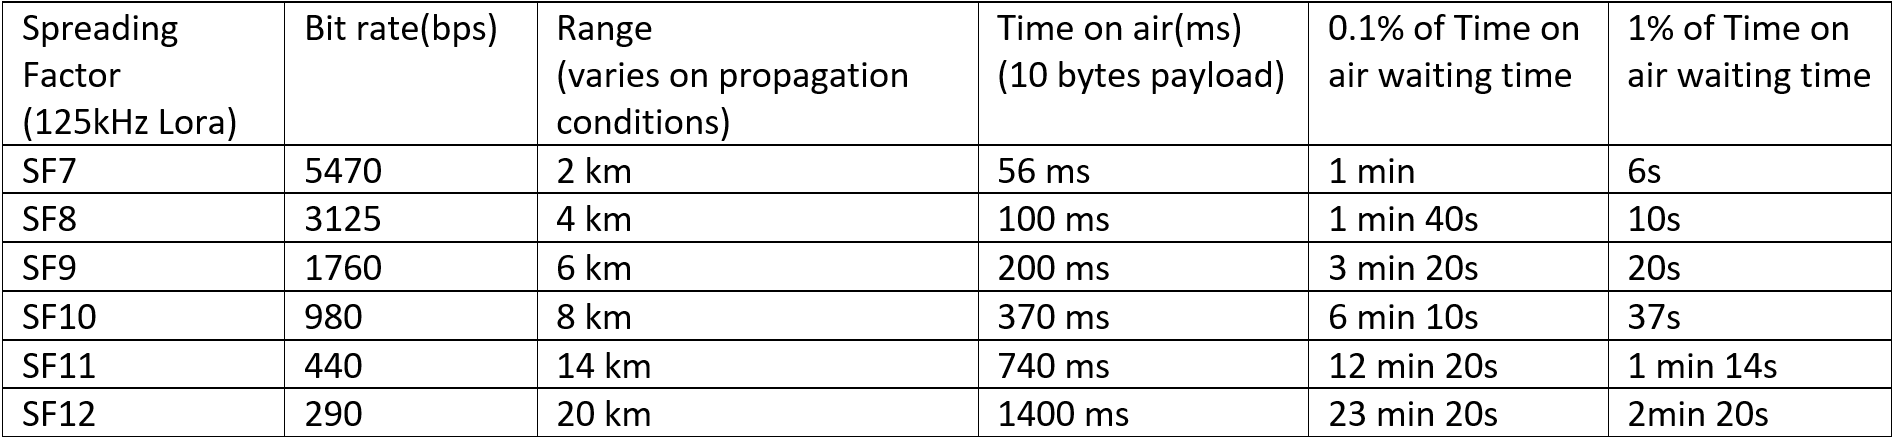
\includegraphics[width=1\textwidth]{spreading_factor_lorawan_2017-07-29}
    \caption{LoRa spread factor options \cite{24}}
    \label{fig:loraSF}
\end{figure}

This technology is very attractive for its long range capability and easy to connect nodes. It's complicated to build a full-capacity gateway which is capable of receiving packets at all frequency channels and SF in parallel. The transceiver for this application costs about \$130. Although it's also possible to build single-channel gateway which is way too cheaper, but it can receive packets at only one frequency channel and SF at once \cite{17} \cite{18} \cite{19} \cite{20} \cite{21} \cite{22} \cite{23} \cite{24}.


\section{Sigfox}
This technology focuses on short message and long range communication applications \cite{25} \cite{26}.


\section{Z-Wawe}
Z-Wave is intended for wireless connectivity for all possible smart home products, controlled by PC, phone, voice, etc. It's based on mesh network topology so every non-battery powered device works as a router to enhance the network range so the more devices are connected in one network, the stronger the network is \cite{27} \cite{28}.


\section{Thread}
This technology based on IPv6 was developed for home network controlled by smartphone, tablet or PC \cite{29} \cite{30} \cite{31}.


\section{RPMA}
The "Random Phase Multiple Access" developed by Ingenu designed for M2M and IoT applications \cite{32} \cite{rpma_ublox} \cite{34}. \textit{"RPMA has been deployed for the Machine Network, but can also be rolled out as a private network installation. It is highly suitable for regions, where the rollout of 3GPP LPWA technologies is lagging, where cellular coverage is generally weak, or where users would like to exert full control over their network deployments."}\cite{rpma_ublox}




% \chapter{Low power wireless network technologies}
todo prepsat do cj

\section{IQRF}
This technology aims to make it easy to implement wireless solutions. It enables peer-to-peer, star and mesh network communication modes. The IQRF alliance provide IQRF transceivers for \$15-20 with a few serial interfaces such as SPI, I2C, UART etc. and they also provide open source SDK which makes it very easy to use IQRF modules. The SDK is based on Java so it's compatible with various platforms such as Linux and Windows
\cite{1} \cite{2} \cite{3} \cite{4}.


\section{Wireless M-bus}
\textit{"Wireless Meter Bus has its origins within the Meter-Bus standards. This is a field bus standard aimed at applications for collecting meter data for gas, electricity, water, etc."} \cite{5}
It supports a few application modes for differing applications.
\begin{itemize}
  \item S1  Unidirectional, data are transmitted only a several times a day.
  \item S2	Bidirectional version of S1.
  \item	T1	Unidirectional transmission of data with a period of a few seconds of minutes.
  \item T2	Bidirectional version of T1.
  \item C1	Unidirectional transmission of bigger amount of data.
  \item C2	Bidirectional version of C1.
\end{itemize}
Usually one M-bus device support only a few of these application modes \cite{5} \cite{6} \cite{7} \cite{8}.


\section{Zigbee}
Zigbee, developed by zigbee alliance is usually used for mesh sensor networks because of its short range. This technology is standardized since 2003, so there is many available nodes at the market by now \cite{10} \cite{11} \cite{12}.

\section{Bluetooth}
Bluetooth has the big advantage, taht it's built in almost every mobile phone, tablet or laptop so there are more options to control the network. The Bluetooth 4.0+ also called BLE (Bluetooth Low Energy) aims to low power wireless sensor networks.
It can be used for point-to-point, broadcast or mesh network topology \cite{13} \cite{14} \cite{15} \cite{16}.


\section{LoRa}
The name LoRa stands for "Long Range" wireless communication with low data rate and power consumption. The protocol enables to modify SF which affects the communication range and data rate. The \ref{fig:loraSF} shows this dependence.

\begin{figure}[!h]
    \centering
    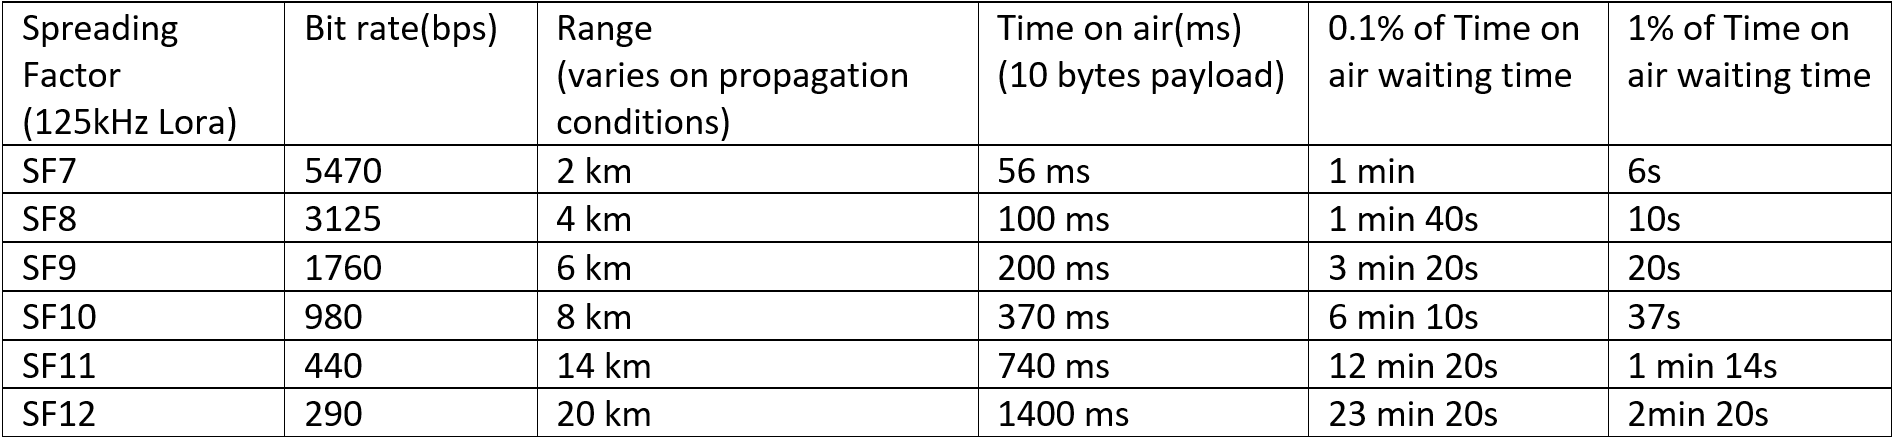
\includegraphics[width=1\textwidth]{spreading_factor_lorawan_2017-07-29}
    \caption{LoRa spread factor options \cite{24}}
    \label{fig:loraSF}
\end{figure}

This technology is very attractive for its long range capability and easy to connect nodes. It's complicated to build a full-capacity gateway which is capable of receiving packets at all frequency channels and SF in parallel. The transceiver for this application costs about \$130. Although it's also possible to build single-channel gateway which is way too cheaper, but it can receive packets at only one frequency channel and SF at once \cite{17} \cite{18} \cite{19} \cite{20} \cite{21} \cite{22} \cite{23} \cite{24}.


\section{Sigfox}
This technology focuses on short message and long range communication applications \cite{25} \cite{26}.


\section{Z-Wawe}
Z-Wave is intended for wireless connectivity for all possible smart home products, controlled by PC, phone, voice, etc. It's based on mesh network topology so every non-battery powered device works as a router to enhance the network range so the more devices are connected in one network, the stronger the network is \cite{27} \cite{28}.


\section{Thread}
This technology based on IPv6 was developed for home network controlled by smartphone, tablet or PC \cite{29} \cite{30} \cite{31}.


\section{RPMA}
The "Random Phase Multiple Access" developed by Ingenu designed for M2M and IoT applications \cite{32} \cite{rpma_ublox} \cite{34}. \textit{"RPMA has been deployed for the Machine Network, but can also be rolled out as a private network installation. It is highly suitable for regions, where the rollout of 3GPP LPWA technologies is lagging, where cellular coverage is generally weak, or where users would like to exert full control over their network deployments."}\cite{rpma_ublox}


 % 	this may be added

% \chapter{The design of the sensor network}
% This chapter describes the design of the sensor network.

\section{Block diagram}
\subsection{Node}
The node as an any device that transmits data in the network. In the star network topology it could be only a sensor or an actuator accessed by the gateway, because there are no routing devices or other. \cite{wsn01}.
\subsection{Gateway}
The gateway handles the communication with all the nodes and transmits the data to other network or device \cite{wsn01}. 
In this case the gateway is accessed by the LAN through RS-485 interface. 
\begin{figure}[!h]
    \centering
    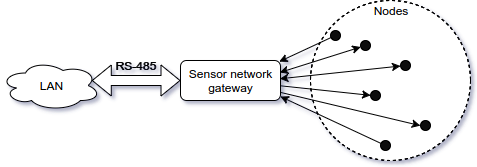
\includegraphics[width=1\textwidth]{LPwSN_bd}
    \caption{The block diagram of the sensor network}
    \label{fig:Typical structure of a card}
\end{figure}


\section{The requirements for the wireless technology}
The main requirement for the designed network is ability to add many various nodes which are available at the market to the network, so we don't have to make our own nodes for every kind of application.
The other requirements are price, power consumption, range etc.


\section{The final choose of the low power wireless technology}
From all the compared technologies in the table in appendix is chosen LoRa, because its nodes are easy to implement to the network with no restrictions. For example there is also many BLE nodes available at the market, but many of manufacturers say that their nodes are compatible only with their own network gateway so it may not be possible to add the node to our designed network. 
To make it simple and cheap only single channel gateway is used which means that all the devices in the network must be configured to one predefined channel and SF. 
															

% \part{Practical part}

\chapter{Účel LPWSN v kontextu současného stavu ve světě}


\chapter{Identifikace problému, který LPWSN řeší}
\chapter{Stanovení požadavků návrhu zařízení}

Cílem tohoto projektu je návrh, realizace a otestování gatewaye, která shromažďuje data z bezdrátových koncových zařízení a přeposílá je přes RS485 LAN na PC master, který je dále přeposílá na IMA K4 server, kde jsou data zpracovávány.

\begin{figure}[!h]
    \centering
    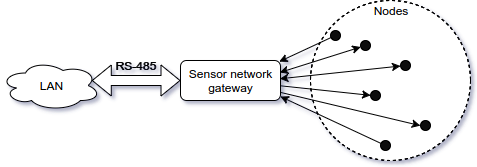
\includegraphics[width=1\textwidth]{01}
    \caption{Blokový diagram funkce gatewaye}
    \label{fig:block diagram of the system}
\end{figure}

Předpokládá se, že koncová zařízení jsou senzory nebo aktuátory napájeny z baterie, tudíž pro jejich dlouhodobou životnost je kladen důraz na nízkou spotřebu vybrané bezdrátové technologie.

Drátová síť RS485, přes kterou gateway komunikuje s PC masterem používá síťový protokol původně navržen pro přístupové systémy. 
Rošiřování vlastností tohoto protokolu by znamenalo mnoho komplikací, cílem je tedy implementace IoT tak, aniž by bylo nutné protokol rozšiřovat.

\section{Přístupové systémy}
Přístupové systémy jsou elektronické systémy řídící skrze síť přístup uživatelů do budov či objektů na základě ověření jejich identity \cite{accessControlSystem_eiprocus}.
V obrázku \ref{fig:Access control system architecture} je znázorněn příklad infrastruktury přístupového systému.

\begin{figure}[!h]
    \centering
    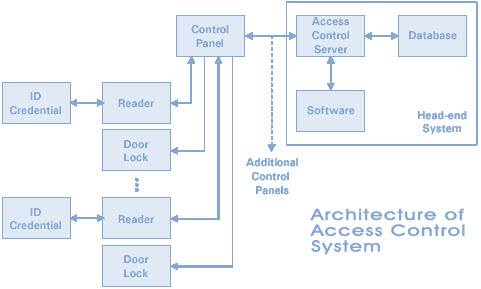
\includegraphics[width=1\textwidth]{Architetcture-of-Access-Control-System}
    \caption{Příklad architektury přístupového systému \cite{accessControlSystem_eiprocus}}
    \label{fig:Access control system architecture}
\end{figure}

todo: popsat jednotlive bloky obrazku

\section{Implementace IoT do přístupového systému firmy IMA}
V použitém systému firmy IMA je control panel nazýván PC Master, který komunikuce s čtečkami proprietárním protokolem přes rozhranní RS485.
Účelem tohoto projektu je tedy nahrad


% todo: 
% - popiste infrastrukturu pristupovych systemu (obrazek a popis jednotlivych bloku), a jednak jejich vyuziti, zda se pouzivaji i na neco jineho - opet clanky, ten obr. 3.1 neni dostatecny pro clanek. Mam na mysli toto:
% https://www.elprocus.com/understanding-about-types-of-access-control-systems/
% https://en.wikipedia.org/wiki/Access_control#Access_control_system_topologies
\chapter{Realizace gatewaye}

\section{Výběr přenosové technologie}
Pro tento systém je použita RF technologie LoRa se standardizovaným síťovým protokolem LoRaWAN, ale s požitím pouze jednoho kanálu.
Jedenokanálové řešení bylo zvoleno z toho důvodu, že plnohodnotný LoRa transceiver, který přijímá na všech osmi kanálech je příliš drahý (přibližně desetinásobná cena) a složitý k implementaci, zatímco v tomto projektu je kladen důraz na cenu a jednoduchost řešení.

Vybraná technologie používá topologii typu hvězda, tedy koncová zařízení komunikují přímo s gatewayí, zbytek času mohou být ve stavu nízké spotřeby, což má za důsledek delší životnost baterie.
Koncová zařízení od různých výrobců jsou plně kompatibilní s cizí gatewayí, tudíž není problém je implementovat do tohoto systému. Je pouze třeba je překonfigurovat pro vysílání na jednom použitém kanále.

% todo: tahle section by mozna mohla byt nekde jinde
% \subsection{Zabezpečení protokolu LoRaWAN}
% Protokol LoRaWAN používá AES-128 na 2 způsoby, pro síťové a aplikační zabezpečení. Jsou zde tedy 2 šifrovací klíče, NwkSKey a AppSKey.

% \subsubsection{Síťové zabezpečení}
% Síťové zabezpečení je zde aby bylo hackerům zabráněno odesílání duplikovaných paketů nebo vytváření a vysílání paketů s nasimulovanými daty.
% Poslední 4 byty paketu obsahují MIC (Message Integrity Code), který je získán zašifrováním dat síťovým klíčem NwkSKey obsahujících mimo jiné celý payload paketu (včetně paket counter). Toto umožňuje odhalit jakoukoliv manipulaci s daty v paketu. LoRaWAN paket také obsahuje counter počítající od nuly od doby kdy bylo LoRaWAN zařízení spuštěno. Toto umožňuje odhalit duplikování paketů.


\subsubsection{Aplikační zabezpečení}
Aplikační klíč AppSKey (Application Session Key) je použit pro zašifrování dat aplikační zprávy (App message) \cite{lwSpec} \cite{lwSecur}.


%%%%%%%%%%%%%%%%%%%%%%%%%%%%%%%%%%%%%%%%%%%%%%%%%%%%%%%%%%%%%%%%%%%%%%%%%%
\section{Výběr komponent}
\subsection{Microcontroller}
Pro toto zařízení je zvolen mikrocontroller STM32L073RZ se zaměřením na nízkou spotřebu, jelikož je levný, má dostačující vlastnosti a je dostupný ve formě vývojového kitu NUCLEO-L073RZ který byl použit pro  vývoj zařízení. Mezi hlavní vlastnosti patří \cite{nucleoST}:
\begin{itemize}    
    \item {Architektura ARM Cortex-M0+ 32-bit RISC}
    \item{Interní Flash paměť 192 KB}
    \item{Interní SRAM paměť 20 KB}
    \item{Interní EEPROM paměť 6 KB}
    \item {Až 32 MHz CPU}
    \item {2X SPI, 3x I2C, 4x USART, LIN, ADC}
\end{itemize}

Pořizovací cena kitu přímo na stránce výrobce www.st.com je \$13 \cite{nucleoST} \cite{nucleoMbed}.
\begin{figure}[!h]
    \centering
    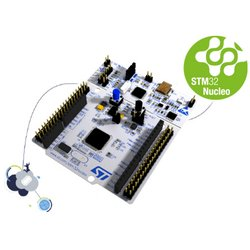
\includegraphics[width=0.4\textwidth]{Nucleo64}
    \caption{Vývojový kit NUCLEO-L073RZ \cite{nucleoST}}
    \label{fig:02}
\end{figure}

\subsection{LoRa transceiver}
Lora transceiver čip doposud vyrábí pouze Semtech, pro použití v Evropském pásmu je určen typ SX1276.
V tomto návrhu je použita deska RFM95w od firmy HopeRF s integrovaným čipem SX1276 \cite{RFM95w}.
Pro vývoj zařízení byl využit tento transciever v tzv. Dragino LoRa Shield \cite{draginoWiki}, který má stejně jako použitý vývojový kit, pinout kompatibilní s Arduino UNO. Pořizovací cena samotného transceiveru RFM95w je okolo \$7, cena Dragino Shieldu se pohybuje okolo \$22 na ebay.

\begin{figure}[!h]
    \centering
    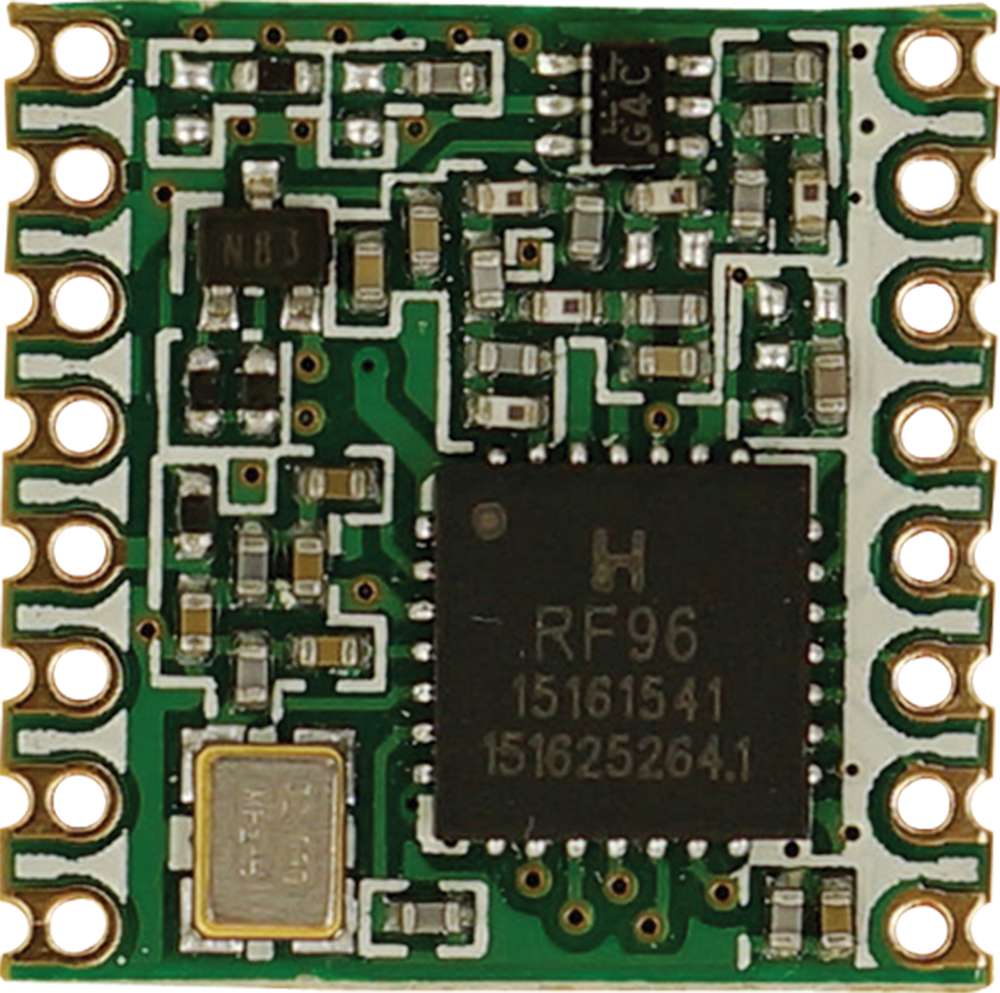
\includegraphics[width=0.2\textwidth]{RFM95w}
    \caption{LoRa transceiver RFM95w \cite{RFM95w}}
    \label{fig:02}
\end{figure}

\subsection{RS485 transceiver}
SparkFun Transceiver Breakout - RS485 převádí rozhranní UART na RS485, pří vstupním napětí 3.3 V. A je dostupný za cenu okolo \$10 \cite{rs485tr}.

\begin{figure}[!h]
    \centering
    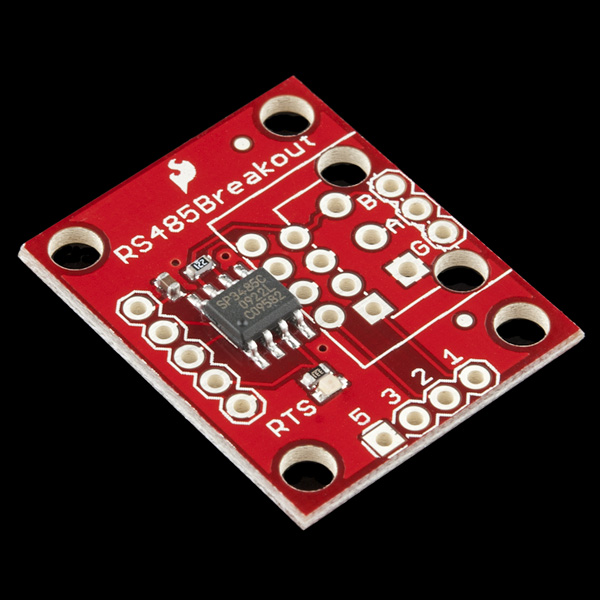
\includegraphics[width=0.4\textwidth]{rs485transceiver}
    \caption{RS485 transceiver \cite{rs485tr}}
    \label{fig:rs485transceiver}
\end{figure}

\newpage
%%%%%%%%%%%%%%%%%%%%%%%%%%%%%%%%%%%%%%%%%%%%%%%%%%%%%%%%%%%%%%%%%%%%%%%%%
\section{Implementace LoRaWAN sítě}
Jednokanálové použití technologie LoRa umožňuje použít transceiver navržený pro koncová zařízení, 
kterým jsou pakety kontinuálně odposlouchávány na jednom nastaveném kanále a SF. Tyto dva parametry  jsou nakonfigurovány na všech koncových zařízeních v síti.

Použitý protokol IMA\_RS485, původně navržen pro přístupové systémy, umožňuje posílat data pouze pomocí příkazu "průchod", který má kapacitu pro data z koncového zařízení pouze 6 B. Systém je proto navržen neobvyklým způsobem. Přijme-li gateway LoRaWAN paket, nejprve zkontroluje zda zná adresu zařízení, pokud ano, přečte z paměti i typ zařízení, paket dešifruje a dekóduje payload, čímž získá konečné hodnoty senzorů, které pak dále pošle přes RS485 rozhraní na master.
LoRaWAN device address a typ každého zařízení v síti je uložena v EEPROM (non-volatile) paměti gatewaye a jsou nastavována na K4 serveru.
Všechna zařízení mají nastavené stejné šifrovací klíče a gateway je má uložené v EEPROM.

Pro tento projekt byla vyvinuta knihovna pro dekódování payloadu na základě dokumentů \cite{lwSpec} \cite{lwSecur}.


%%%%%%%%%%%%%%%%%%%%%%%%%%%%%%%%%%%%%%%%%%%%%%%%%%%%%%%%%%%%%%%%%%%%%%%%%%
\section{Implementace komunkičního protokolu v síti IMA\_RS485}
V tomto projektu je komunikace protokolu IMA\_RS485 naprogramována v souborech rs485\_protocol.h a rs485\_protocol.c. Jedná se o kolizní protokol v síti, kde je připojen jeden master, a jeden nebo více slaveů řízených masterem.

\begin{table}[!h]
    \centering
    \begin{tabular}{ |c|c| }
     \hline

     Baud rate              & 9600           \\ \hline
     Data bits              & 8                 \\ \hline
     Parity                 & none              \\ \hline
     Stop bits              & 1                 \\ \hline

    \end{tabular}
    \caption{Fyzické vlastnosti IMA\_RS485 sítě}
    \label{table:3}
\end{table}

\newpage
\subsection{Syntaxe příkazů}
Komunikace v síti probíhá formou příkazů, které mají specifikovanou syntaxi v tabulce \ref{table:syntaxePrikazu}.

\begin{table}[!h]
    \centering
\begin{tabular}{ |c|| p{1.5cm} | p{1.5cm} | p{1cm} | p{1cm} | p{1cm} | p{1cm} | }
 \hline
 popis      & adresa příjemce & adresa odesílatele & typ příkazu & délka dat & data & crc\\ \hline
 počet bytů & 1               & 1   & 1     & 2     & délka dat     & 1 \\ 
 \hline
\end{tabular}
    \caption{Syntaxe příkazu pro komunikaci v síti IMA\_RS485}
    \label{table:syntaxePrikazu}
\end{table}

Typy příkazu jsou zadefinované konstanty s předponou CKP\_CMD\_ v souboru ./Inc/rs485\_protocol.h.
Příkazy odeslané masterem obsahují navíc synchronizační byte na začátku 0xAA.
CRC je pro kontrolu XOR přes všechny předchozí byty v celém příkazu kromě synchronizačního bytu.

\subsection{Adresace zařízení v síti}
Každé zařízení na této sběrnici má svoji adresu, která mu je nastavena externě. Master má adresu  0xFF, adresa pro všechny (broadcast) je 0x00 a zařízení v této sítí můžou mít adresu libovolnou (krom těchto dvou) nesmí zde však být připojena 2 zařízení s nastavenou stejnou adresou.

\subsection{Statusy}
Slave má dva možné statusy, offline a online, což značí, zda je zařízení v aktivním režimu, tudíž má povolení odesílat příkaz průchod (V případě této gatewaye příkaz průchod obsahuje data ze koncového zařízení).  
Slave odesílá příkaz obsahující informaci o jeho statusu periodicky s typem příkazu 0x10 a jedním bytem dat označujícím status. Master na tento příkaz odpoví pouze pokud mění status slaveu. Pokud je slave online a master přestane komunikovat, zařízení slave se samo přepne na status offline.

\subsubsection{Offline}
Je-li zařízení zapnuto, je ve stavu offline. Nemá povoleno odesílat příkaz průchod obsahující data z koncových zařízení, pouze odpovídá na příkazy masteru. Odesílání příkazu signalizující tento stav je s periodou 10 s a obsahuje byte 0xEE.

\subsubsection{Online}
Odesílání příkazu signalizující tento stav je s periodou 45 s a obsahuje byte 0x00.
V tomto stavu je povoleno odesílání příkazu průchod.


\subsection{Přidávání LoRaWAN zařízení do systému}
Pokud master přijme od slavea příkaz oznamující že je ve stavu offline, nejprve slaveu pošle seznam LoRaWAN adres všech známých koncových zařízení a následně slavea přepne do stavu online.
Přijímání seznamu adres je realizováno sekvencí příkazů typu 0x8F. 

Níže v tabulce \ref{table:2} je příklad sekvence příkazů odesílaných mezi masterem a slavem během předávání seznamu LoRaWAN device address koncových zařízení, kde slave má adresu 0x10 a master standardně 0xFF. Jak již bylo řečeno, příkazy od masteru lze jednoduše odlišit tím, že vždy začínají bytem 0xAA.


\begin{table}[!h]
    \begin{tabular}{ |l|p{10cm}| }
    \hline
    příkaz      &  data    \\ \hline \hline
    master: start      &  AA 10 FF 8F 02 00 00 00 62    \\ \hline
    slave: ACK        &  FF 10 06 02 00 8F 00 64    \\ \hline
    master: data     &  AA 10 FF 8F 21 00 01 B1 C4 12 00 00 00 00 00 B2 C4 12 00 00 00 00 00 B3 C4 12 00 00 00 00 00 B4 C4 12 00 00 00 00 00 44 \\ \hline
    slave: ACK      &  FF 10 06 02 00 8F 01 65   \\ \hline
    master: data     &  AA 10 FF 8F 19 00 02 B5 C4 12 00 00 00 00 00 B6 C4 12 00 00 00 00 00 F6 1F 01 26 00 00 00 00 B6 \\ \hline
    slave: ACK      &   FF 10 06 02 00 8F 02 66   \\ \hline
    master: konec   &   AA 10 FF 8F 04 00 03 FF 2A 57 E5   \\ \hline
    slave: ACK      &   FF 10 06 02 00 8F 03 67  \\ \hline
    \end{tabular}
    \caption{Příklad sekvence příkazů odesílaných mezi masterem a slavem během předávání seznamu LoRaWAN device address koncových zařízení}
    \label{table:2}
\end{table}

LoraWAN protokol používá 4-bytové adresy koncových zařízení.
Adresy předávány touto sekvencí jsou dlouhé 8-bytové. První 4 byty je tedy LoRaWAN device address, pátý byte je typ zařízení a zbylé 3 byty jsou nevyužity, jejich použití je možné v případě změn či rozšiřování vlastností systému. 

První Byte dat je counter paketu začínající od nuly, který označuje číslo odeslaného paketu v sekvenci. Na každý tento paket v sekvenci slave odpovídá ACK příkaz, který se liší od obyčejného ACK příkazu tím, že v datech paketu navíc obsahuje counter pakety v sekvenci.
První příkaz této sekvence má délku dat 2 byty, které mají hodnotu 0x00 přičemž první je counter.
Další příkazy hned za counter bytem obsahují několik osmibytových adres, jejichž počet je různý.
Příkaz ukončující tuto sekvenci příkazů má délku 4 byty, což je tedy counter, 0xFF a 2 byty CRC přes všechny odeslané adresy (nepodstatné, tudíž ho nepoužívám).

\subsection{Odesílání dat z koncových zařízení}
Jak již bylo zmíněno, protokol byl navrhnut pro přístupové systémy, tudíž data z koncových zařízení jsou odesílána příkazem "průchod", jehož typ je 0x10 a kapacita na data z koncového zařízení je pouze 6 B. 

První byte dat označuje typ průchodu, byl zvolen konstantní byte 0xD0. Dále následuje LoRaWAN adresa koncového zařízení od kterého byl paket přijat. Dále následují 4 byty dat ze senzoru, další 2 byty signalizující čas průchodu, což v tomto projektu není použito a tyto dva byty mají vždy hodnotu 0xFF. A nakonec jsou další 2 byty obsahující data ze senzoru.

Příklad příkazu: FF 1F 10 0D 00 D0 F6 1F 01 29 AD 0A 5A 27 FF FF DE 09 E1.

Data příkazu jsou níže rozepsána v tabulce \ref{table:prikladprikazpruchod}.

\begin{table}[!h]
    \centering
\begin{tabular}{ | p{1.5cm} | p{3cm} | p{2.5cm} | p{1.3cm} | p{1.3cm} |  }
 \hline
 typ průchodu & LoRaWAN device address & data (4B)     & cas   & data (2B) \\ \hline
 D0           & F6 1F 01 29            &  AD 0A 5A 27  & FF FF & DE 09     \\ 
 \hline
\end{tabular}
    \caption{Příklad dat příkazu "průchod" odeslaného z gatewaye k masteru, obsahující data z koncových zařízení}
    \label{table:prikladprikazpruchod}
\end{table}

Master na příkaz "průchod" odpovídá příkazem ACK. Slave na tuto odpověď čeká standardně 3 sekundy, ale tento parametr je nastavitelný. Pokud v tomto timeoutu master neodpoví, slave  příkaz zopakuje a změní typ příkazu na 0x20. Pokud master ani na třetí opakování neodpoví ACK, slave se přepne do stavu offline a vymaže frontu příkazů "průchod" k odeslání.

\subsection{Potvrzení}
Slave odpovídá na každý příkaz od masteru ACK. Typ příkazu ACK je 0x06 a data příkazu obsahují jeden byte signalizující typ příkazu na který je právě odpovídáno potvrzením.
Master odpovídá ACK se stejným typem příkazu 0x06, ale s žádnými daty příkazu.

\subsection{Dotaz na příznaky}
Master se může zeptat s jak dlouhými adresami slave pracuje s typem příkazu 0x49. Slave na to odpovídá ACK s tím, že v datech příkazu je navíc byte 0x04. Master pak počítá s tím, že slave pracuje se 64-bit adresami (ve skutečnosti ale používá 32-bitové a zbylé 4 byty v příkazu průchod jsou pro data z koncového zařízení).

%%%%%%%%%%%%%%%%%%%%%%%%%%%%%%%%%%%%%%%%%%%%%%%%%%%%%%
\section{Komunikace přes USB}
Gateway má implementovanou komunikaci přes USB, což má za účel konfiguraci systému a logování. K přípojení přes USB lze použít PC s  aplikací terminálu s nastavením viz tabulka \ref{table:usb_term}.

\begin{table}[!h]
    \centering
    \begin{tabular}{ |c|c| }
     \hline

     Baud rate              & 115200           \\ \hline
     Data bits              & 8                 \\ \hline
     Parity                 & none              \\ \hline
     Stop bits              & 1                 \\ \hline
     Flow control           & none               \\ \hline

    \end{tabular}
    \caption{Nastavení USB terminálu}
    \label{table:usb_term}
\end{table}

Při komunikaci jsou data standardně oddělována bytem CR (carriage return) 0x0D, ale je akceptována i sekvence CR LF (Line Feed), tedy 0x0D 0x0A. 

%%%%%%%%%%%%%%%%%%%%%%%%%%
\subsection{Log aplikace}
Gateway loguje informace o proběhlých událostech přes USB. 
Níže je příklad výpisu dat pro případ, že gateway přjala LoRaWAN paket z koncového zařízení v síti.

Nejprve jsou vypsána data týkající se LoRaWAN protokolu, zašifrovaný i dešifrovaný payload, typ zařízení a konečné informace dekódované z payloadu.
Poslední řádek začínajci s předponou "Tx -> RS-485:" obsahuje data odeslané k masteru přes RS485 síť.

todo: nakopirovat priklad aktualizovaneh vypisu dat
\begin{lstlisting}
______________________________________________________
Rx -> LoRaWAN, pktCntr: 406
RSSI: -29, SNR: 9, length: 22
paket rawData:  40 F6 1F 01 26 C0 A1 30 08 D4 5D 93 F0 F0 F6 60 C0 04 BC BE 4B 24
devAddr:  F6 1F 01 26
MHDR: 40
FCtrl: c0
FCnt: 12449
FPort: 08
MIC:  BC BE 4B 24
adaptive data rate:  1
ack: 0
direction: UP
message (encrypted):  D4 5D 93 F0 F0 F6 60 C0 04
message (decrypted):  01 44 6C 83 05 00 FF FF 71

Sensor type: RHF1S001
temperature: 27.46 C, humidity: 58 %
period: 10 s, RSSI: -29 dBm, SNR: 9 dB, battery voltage: 2.6 V
Tx -> RS-485: "FF 10 10 0D 00 D0 F6 1F 01 26 BA 0A 3A E3 FF FF 09 1A 96"
\end{lstlisting}

%%%%%%%%%%%%%%%%%%%%%%%%%%
\subsection{Konfigurace systému}
\label{sec:konfigurace}
Konfigurace gatewaye se provádí opět přes USB port. Je do ní vstoupeno odesláním příkazu
"config", následuje vypsání současného stavu konfigurace a dále je vypsáno konfigurační menu, kde uživatel vybere jednotlivý bod menu zadáním jeho čísla na začátku řádku.
Níže je zobrazen příklad výpisu po vstupu do konfigurace.

\begin{lstlisting}
    _________________Entering configuration setup________________
    
    System configuration:
    
    *** LoRa channel: 
    channel: 0 (868.1 Mhz)
    SF7
    
    *** RS485 channel: 
    my address: 10
    master address: FF
    timeout: 3 s
    
    *** LoRaWAN keys: 
    NwSKey:  FD 90 0D 8C 70 9F 19 24 18 EC FD D4 28 0C AC 47
    AppSKey:  68 9F D0 AC 7A 0F 95 58 B1 19 A0 16 17 F4 16 33
    
    
    Config menu:
    1 -> Config LoRa channel
    2 -> Config RS485 channel
    3 -> Config LoRaWAN protocol
    4 -> Print all LoRaWAN devices
    5 -> Erase all LoRaWAN devices
    6 -> Restore to default configuration
    7 -> Exit without save
    8 -> Save and exit
\end{lstlisting}
    

Z konfigurace je možné vystoupit kdykoliv bez uložení změn příkazem "quit". 
Při vstoupení do konfigurace je pozastavena činnost gatewaye, komunikace s koncovými zařízeními LoRaWAN síťě a komunikace s masterem v síti RS485 nejsou aktivní.
Jsou zde tedy 3 stavy konfigurace, přičemž je možné vždy jednotlivá nastavení přeskakovat odesláním "prázdného příkazu" 0x0D (v terminálu obvykle stačí stisknout Enter). Systém při konfiguraci vždy vypíše jaká data mají být zadána v jakém tvaru a zároveň současnou hodnotu měněného parametru. Zadaná data uživatelem jsou vždy zkontrolována zda splňují požadovaný tvar. Pokud ne, uživatel je o tom informován a vyzván k dalšímu pokusu.
Po provedení konfigurace následuje vždy návrat zpět do hlavního menu. Pro uložení nové konfigurace je potřeba v menu vybrat "Save and exit", gateway pak následně vypíše které parametry byly změněny a provede restart.

\subsubsection{Config LoRa channel}
Konfigurace LoRa RF kanálu zahrnuje nastavení SF a frekvenční pásmo. Níže je příklad konfigurace.

\begin{lstlisting}
LoRa channel configuration:
Enter SF number (7-12)
(current: 7)
8
SF8 set.

Enter LoRa channel number (0-7)
ch0 is 868.1 Mhz
ch1 is 868.3 Mhz
ch2 is 868.5 Mhz
ch3 is 867.1 Mhz
ch4 is 867.3 Mhz
ch5 is 867.5 Mhz
ch6 is 867.7 Mhz
ch7 is 869.0 Mhz
(current: 0)
1
channel 1 set.
\end{lstlisting}

\subsubsection{Config RS485 channel}
Konfigurace RS485 kanálu pro komunikaci s masterem zahrnuje nastavení adresy tohoto zařízení, adresa masteru a timeout, což je doba čekání na potvrzení od masteru po odeslání příkazu "průchod". Níže je příklad konfigurace.

\begin{lstlisting}
RS485 channel configuration:
Enter address of this device, FF and 00 are reserved.
(current: 10)
11
Address of this device is set to: 11

Enter master address: 
(current: FF)
FE
Master address is set to: FE

Enter timeout (seconds)
(current: 3)
5
timeout set to: 5 s
\end{lstlisting}


\subsubsection{Config LoRaWAN protocol}
Konfigurace LoRaWAN protokolu zahrnuje nastavení šifrovacích klíčů NwkSKey a AppSKey. Níže je příklad konfigurace.

\begin{lstlisting}
LoRaWAN protocol configuration:
Enter NwkSKey (16 bytes in HEX)
(current:  FD 90 0D 8C 70 9F 19 24 18 EC FD D4 28 0C AC 47)
11111111222222223333333344444444
NwSKey set to: 11 11 11 11 22 22 22 22 33 33 33 33 44 44 44 44

Enter AppSKey (16 bytes in HEX)
(current:  68 9F D0 AC 7A 0F 95 58 B1 19 A0 16 17 F4 16 33)
11111111222222223333333344444444
AppSKey set to: 11 11 11 11 22 22 22 22 33 33 33 33 44 44 44 44
\end{lstlisting}


\subsubsection{Print all LoRaWAN devices}
Vypíše všechna LoRaWAN zařízení uložená v paměti. Níže je příklad.


\begin{lstlisting}
number.......................0:
Device Address:  B1 C4 12 00
Device Type: RH1S001
number.......................1:
Device Address:  B2 C4 12 00
Device Type: RH1S001
number.......................2:
Device Address:  B3 C4 12 00
Device Type: RH1S001
number.......................3:
Device Address:  B4 C4 12 00
Device Type: IMA_tempPress
number.......................4:
Device Address:  B5 C4 12 00
Device Type: IMA_tempPress
\end{lstlisting}



\subsubsection{Restore default configuration}
Po zvolení této možnosti je načtena defaultní konfigurace systému, která obsahuje hodnoty viz tabulka \ref{table:5}. Tyto defaultní hodnoty jsou nastaveny v programu a slouží především pro testovací účely.

\begin{table}[!h]
    \centering
    \begin{tabular}{ |l|l| }
     \hline

     popis              & hodnota         \\ \hline \hline
     RS485 myAddr       & 0x10            \\ \hline
     RS485 MasterAddr   & 0xFF            \\ \hline
     RS485 timeout      & 3               \\ \hline
     LoRa SF            & SF7             \\ \hline
     LoRa channel       & 0 (868.1 Mhz)   \\ \hline
     NwSKey             & FD 90 0D 8C 70 9F 19 24 18 EC FD D4 28 0C AC 47  \\ \hline
     AppSKey            & 68 9F D0 AC 7A 0F 95 58 B1 19 A0 16 17 F4 16 33  \\ \hline

    \end{tabular}
    \caption{Defaultní konfigurace systému}
    \label{table:5}
\end{table}


\newpage
%%%%%%%%%%%%%%%%%%%%%%%%%%%%%%%%%%%%%%%%%%%%%%%%%%%%%%
\section{Koncová zařízení}
Jelikož používaný protokol ke komunikaci s masterem je omezen na pouhých 6 B na jeden paket, payload koncových zařízení je dekódován v gatewayi a v paketu odeslaném na master jsou pouze vybraná nejdůležitější data, která se vejdou do této velikosti.
Prote společně s LoRaWAN device address koncového zařízení je v gatewayi uložen i typ zařízení zadefinován jedním bytem a na základě typu zařízení gateway rozpozná jak dekódovat payload.

Momentálně jsou podporovány dva typy koncových zařízení, dle potřeby je možné rozšířit FW gatewaye o další typy koncových zařízení.

\begin{table}[!h]
    \centering
    \begin{tabular}{ |l|l| }
     \hline

     Typ zařízení       & Hodnota         \\ \hline \hline
     RHF1S001           & 0x00            \\ \hline
     IMA\_tempPress     & 0x01            \\ \hline
     
    \end{tabular}
    \caption{Typy koncových zařízení}
    \label{table:TypyKoncZarizeni}
\end{table}

\subsection{Zpracování dat jednotlivých typů koncových zařízení}
Níže je popsáno pro jednotlivá podporovaná koncová zařízení jak jsou data uložena v datové struktuře, jak jsou data z této struktury zpracována a zobrazena a nakonec jak vybraná data jsou zapsána do výsledného bufferu o délce 6 B, který je odeslán do masteru příkazem "průchod".

\subsubsection{RHF1S001}
Senzor od firmy RisingHF měří teplotu a vlhkost.

\begin{lstlisting}[style=CStyle]
    /* RHF1S001 data structure */   
    typedef struct {
        int16_t temperature;
        uint8_t humidity;
        uint16_t period;
        int8_t rssi;
        int8_t snr;
        uint8_t battery;
    } RHF1S001_data_t;

    /* Print the data from the structure */
	printf("temperature: %d.%d C, ", RHF1S001_data.temperature / 100, RHF1S001_data.temperature % 100);
	printf("humidity: %d %%\n", RHF1S001_data.humidity);
	printf("period: %d s, ", (int)RHF1S001_data.period);
	printf("RSSI: %d dBm, ", RHF1S001_data.rssi);
	printf("SNR: %d dB, ", RHF1S001_data.snr);
	printf("battery voltage: %d.%d V\r\n", RHF1S001_data.battery/10, RHF1S001_data.battery % 10);

    /* Put the data into 6B long buffer, that is transmitted to the master */
	buffer[0] = RHF1S001_data.temperature & 0xFF;
	buffer[1] = RHF1S001_data.temperature >> 8;
	buffer[2] = RHF1S001_data.humidity;
	buffer[3] = RHF1S001_data.rssi;
	buffer[4] = RHF1S001_data.snr;
	buffer[5] = RHF1S001_data.battery;
\end{lstlisting}


\subsubsection{IMA\_tempPress}
Senzor vytvořený ve firmě IMA, měřící teplotu a tlak.

\begin{lstlisting}[style=CStyle]
    /* IMA_tempPress data structure */   
    typedef struct {
        int16_t temperature;
        uint16_t pressure;
        int8_t rssi;
        int8_t snr;
    } IMA_tempPress_data_t;
    
    /* print the data from the structure */
	printf("temperature: %d.%d C, ", IMA_tempPress_data.temperature / 100, IMA_tempPress_data.temperature % 100);
	printf("pressure: %d.%d Pa\r\n", IMA_tempPress_data.pressure/10, IMA_tempPress_data.pressure % 10);
	printf("RSSI: %d dBm, SNR: %d dB\r\n", IMA_tempPress_data.rssi, IMA_tempPress_data.snr);

    /* Put the data into 6B long buffer, that is transmitted to the K4 server */
	buffer[0] = IMA_tempPress_data.temperature & 0xFF;
	buffer[1] = IMA_tempPress_data.temperature >> 8;
	buffer[2] = IMA_tempPress_data.pressure & 0xFF;
	buffer[3] = IMA_tempPress_data.pressure >> 8;
	buffer[4] = IMA_tempPress_data.rssi;
	buffer[5] = IMA_tempPress_data.snr;
\end{lstlisting}


\subsection{Přidávání koncových zařízení ze serveru K4}
Koncocová zařízení sítě se nastavují ze serveru K4 v podobě seznamu offline karet s délkou UID 8 B.
LoRaWAN device address je dlouhá 4 B, jeden byte je navíc použit pro typ koncového zařízení, zbylé 3 byty jsou nuly.
Jelikož typ zařízení je uložen v gatewayi i na K4 serveru. Při odesílání příkazu průchod se tedy už typ zařízení neposílá z důvodu datového omezení tohoto příkazu.
Na serveru K4 se UID nastavuje jako dekadické číslo.
Níže je příklad vytvoření výsledného čísla obsahující DevAddr a typ zařízení, které se zadává do K4 serveru.

\subsubsection{Příklad}
Pro případ, kde typ zařízení je 01 a DevAddr AABBCCDD (little endian) výsledné číslo v hexadecimální podobě je 01DDCCBBAA. Následně se překládá do decimalni podoby, výsledné číslo k zadání do K4 serveru je tedy 8016149418.


%%%%%%%%%%%%%%%%%%%%%%%%%%%%%%%%%%%%%%%%%%%%%%%%%%%%%%
\section{Využití non-volatile paměťi gatewaye}
Konfigurace a adresy s typy všech koncových zařízení v LoRaWAN síti jsou uloženy v non-volatile paměti EEPROM gatewaye o kapacitě 6144 B. 
Paměť je tedy rozdělená tak, že od adresy 0 až po 6080 je prostor pro ukládání LoRaWAN zařízení a od 6080 až po 6144 je prostor pro ukládání konfigurace gatewaye.

Každé LoRaWan zařízení v síti má v paměti uložené LoRaWAN device address (4 byty), typ zařízení (1 byte) a další 3 byty jsou rezervovány. 
Jedno koncové zařízení v paměti tedy zabírá  8 B, takže gateway má kapacitu paměti pro až 760 koncových zařízení.


%%%%%%%%%%%%%%%%%%%%%%%%%%%%%%%%%%%%%%%%%%%%%%%%%%%%%%
\section{Zapojení}
LoRa shield \cite{draginoWiki} je nasazen přímo na vývojový kit Nukleo. Kit neobsahuje ISCP konektor, který je součástí pinoutu Arduino UNO a LoRa shield má SPI piny MISO a MOSI přivedeny právě na tento konektor. Musí být tedy propojeny externě viz obrázek \ref{fig:03}. Jumpery na Dragino LoRa shieldu musí také být stejně jako v obrázku.

\begin{figure}[!h]
    \centering
    \includegraphics[width=1\textwidth]{foto01}
    \caption{foto zapojení}
    \label{fig:03}
\end{figure}

Pro komunikaci s LoRa transceiverem je tedy použito SPI1, pro komunikaci přes USB je použito USART2 a pro komunikaci přes RS485 je použito UART1.

\begin{table}[h]
    \centering
    \begin{tabular}{ |c|c|c| }
     \hline

     Periférie          & Název pinu & Pin procesoru           \\ \hline \hline
     
                        & RX  &   PC1            \\
    RS485 transceiver   & TX  &   PC0       \\
                        & RTS  &  PB1      \\     \hline

                        & CS    &  PB6             \\
                        & CLK   &  PA5        \\
   LoRa transceiver     & MISO  &  PA6     \\
                        & MOSI  &  PA7        \\
                        & RST   & PC7          \\
                        & DIO0  & PA10         \\
                        \hline

    \end{tabular}
    \caption{Pinout připojení externích periférií k procesoru}
    \label{table:3}
\end{table}

%%%%%%%%%%%%%%%%%%%%%%%%%%%%%%%%%%%%%%%%%%%%%%%%
\section{Naprogramování}
K naprogramování MCU byla použita HAL knihovna a inicializační nástroj STM32CubeMX poskytnuté výrobcem, tedy ST Microelectronics.
Zdrojové soubory programu byly vyvíjeny v textovém editoru VS-Code, ke kompilaci zdrojových souborů byl použit kompilátor arm-none-eabi-gcc a jako pomocný nástroj makefile skript. 

\subsection{Zdrojové soubory projektu}
Pro šifrování LoRaWAN paketu byla použita knihovna AES-128, dostupná na githubu \cite{AESlib} a knihovna OpenPANA také dostupná z githubu \cite{CMAClib}.
Níže je seznam zdrojových souborů.

\begin{figure}[!h]
    \dirtree{%
        .1 Drivers \DTcomment{STM32 Drivers}.
        .1 Inc\DTcomment{Headers}.
            .2 aes.h\DTcomment{AES-128 library for LoRaWAN paket encryption}.
            .2 cmac.h\DTcomment{library for CMAC calculation in LoRaWAN protocol}.
            .2 LinkedList\_ByteArray.h \DTcomment{Byte array linked list library for stacks}.
            .2 LoRaWAN\_paket.h\DTcomment{LoRaWAN library for paket data decoding}.
            .2 stm32l0xx\_hal\_conf.h\DTcomment{HAL initialization of peripherals}.
            .2 ByteArray.h\DTcomment{Library for Byte array operations}.
            .2 LoRa.h\DTcomment{Library for interfacing LoRa transceiver}.
            .2 main.h\DTcomment{Main file}.
            .2 stm32l0xx\_it.h\DTcomment{HAL initialization of peripherals}.
            .2 eeprom.h\DTcomment{Library for eeprom operations}.
            .2 LoRa\_sensors.h\DTcomment{Library for decoding data from payload}.
            .2 rs485\_protocol.h\DTcomment{Library for RS485 IMA protocol}.
            .2 usb.h \DTcomment{Library for USB communication and system configuration}.
        .1 Src\DTcomment{Sources}.
            .2 aes.c \DTcomment{source file to the aes.h}.
            .2 aes.c \DTcomment{source file to the cmac.h}.
            .2 LinkedList\_ByteArray.c \DTcomment{source file to the LinkedList\_ByteArray.h}.
            .2 LoRaWAN\_paket.c  \DTcomment{source file to the LoRaWAN\_paket.h}.
            .2 stm32l0xx\_hal\_msp.c \DTcomment{HAL source file}.
            .2 ByteArray.c  \DTcomment{source file to the ByteArray.h}.
            .2 LoRa.c \DTcomment{source file to the LoRa.h}.
            .2 main.c \DTcomment{main source file}.
            .2 stm32l0xx\_it.c \DTcomment{HAL source file}.
            .2 eeprom.c \DTcomment{source file to the eeprom.h}.
            .2 LoRa\_sensors.c \DTcomment{source file to the LoRa\_sensors.h}.
            .2 rs485\_protocol.c  \DTcomment{source file to the rs485\_protocol.h}.
            .2 system\_stm32l0xx.c \DTcomment{HAL source file}.
            .2 usb.h \DTcomment{source file to the usb.h}.
    }
\end{figure}


\subsection{Nahrání programu do MCU}
Výstupem kompilace je soubor s koncovkou .binary, který je nahrán do MCU. K tomuto nahrání není potřeba žádný speciální SW nebo HW.
Stačí kit připojit k PC přes USB, v PC se kit zobrazí jako flash disk. Zkompilovaný program s koncovkou .binary stačí překopírovat na toto zařízení. 
Po dobu kopírování souboru bliká na kitu LED1 červená/zelená. Jakmile kopírování skončí, program na kitu je spuštěn, případně je možné kit resetovat černým tlačítkem reset.
Pro uvedení Gatewaye do provozu je nutné se připojit k zařízení přes USB a nastavit všechny parametry viz sekce \ref{sec:konfigurace}.

\bibliographystyle{amsalpha}
% \bibliography{0main}	% not used
% \bibliographystyle{csn690}
\bibliography{mybibliographyfile}
\begin{thebibliography}{9}
%%%%%%%%%%%%%%%%%%%%%%%%%%%%%%%%%%%%%%%%%%%%%%%%%%%%%%%%%%%%%%%

\bibitem[1]{1}
\textit{
RF.
}
IQRF Alliance.

[Online]. Available:
\url{
https://www.iqrf.org/technology/rf
}
[Accessed: 9-Jun-2018].

%___________________

\bibitem[2]{2}
\textit{
IQRF SDK.
}
IQRF Alliance.
[Online]. Available:
\url{
https://www.iqrf.org/technology/iqrf-sdk
}
[Accessed: 9-Jun-2018].

%___________________


\bibitem[3]{3}
\textit{
Transceivers.
}
IQRF Alliance.

[Online]. Available:
\url{
https://www.iqrf.org/products/transceivers
}
[Accessed: 9-Jun-2018].

%___________________

\bibitem[4]{4}
\textit{
IQRF SDK.
}
IQRF Alliance.
[Online]. Available:
\url{
https://www.iqrf.org/technology/iqrf-sdk
}
[Accessed: 9-Jun-2018].

%___________________

\bibitem[4]{4}
\textit{
Three security levels in new IQRF OS 4.0.
}
IQRF Alliance.
[Online]. Available:
\url{
https://www.iqrfalliance.org/news/117-three-security-levels-in-new-iqrf-os-4-0
}
[Accessed: 9-Jun-2018].

%___________________

\bibitem[5]{5}
\textit{
Wireless Meter Bus, WM-Bus Technology.
}
Radio-Electronics.
[Online]. Available:
\url{
http://www.radio-electronics.com/info/wireless/wireless-m-bus/basics-tutorial.php
}
[Accessed: 9-Jun-2018].

%___________________

\bibitem[6]{6}
\textit{
Wireless M-Bus in Industrial Wireless Sensor Networks.
}
Radiocrafts.
[Online]. Available:
\url{
https://radiocrafts.com/technologies/wireless-m-bus-technology-overview/
}
[Accessed: 9-Jun-2018].

%___________________


\bibitem[7]{7}
Radiocrafts: 
\textit{
WirelessM-Bus in Industrial Sensor Networks.
}
[Online]. Available:
\url{
https://radiocrafts.com/uploads/AN024_Using_Wireless_M-BUS_in_Industrial_Sensor_Networks_1_0.pdf
}
[Accessed: 9-Jun-2018].

%___________________

\bibitem[8]{8}
Silicon labs: 
\textit{
WIRELESS M-BUS SOFTWARE IMPLEMENTATION.
}
[Online]. Available:
\url{
https://www.silabs.com/documents/public/application-notes/AN451.pdf
}
[Accessed: 9-Jun-2018].

%___________________

\bibitem[9]{9}
Compass security:
\textit{
Wireless M-Bus Security Whitepaper Black Hat USA 2013.
}
June 30th. 2013, v1.01.
[Online]. Available:
\url{
https://www.compass-security.com/fileadmin/Datein/Research/Praesentationen/blackhat_2013_wmbus_security_whitepaper.pdf
}
[Accessed: 9-Jun-2018].

%___________________

\bibitem[10]{10}
\textit{
Zigbee.
}
Wikipedia.
[Online]. Available:
\url{
https://en.wikipedia.org/wiki/Zigbee
}
[Accessed: 9-Jun-2018].

%___________________


\bibitem[11]{11}
Xueqi Fan, Fransisca Susan, William Long, Shangyan Li: 
\textit{
Security Analysis of Zigbee.
}
May 18, 2017.
[Online]. Available:
\url{
https://courses.csail.mit.edu/6.857/2017/project/17.pdf
}
[Accessed: 9-Jun-2018].

%___________________



\bibitem[12]{12}
\textit{
The Zigbee Alliance.
}
Zigbee alliance.
[Online]. Available:
\url{
http://www.zigbee.org/zigbee-for-developers/about-us/
}
[Accessed: 9-Jun-2018].

%___________________	bluetooth


\bibitem[13]{13}
\textit{
Bluetooth sensor network.
}
mikroelektronika.
[Online]. Available:
\url{
https://www.mikroe.com/blog/bluetooth-sensor-network
}
[Accessed: 9-Jun-2018].

\bibitem[14]{14}
\textit{
Dispelling Common Bluetooth Misconceptions.
}
Sans technology institute.
[Online]. Available:
\url{
https://www.sans.edu/cyber-research/security-laboratory/article/bluetooth
}
[Accessed: 9-Jun-2018].

\bibitem[15]{15}
\textit{
Bluetooth radio interface, modulation, \& channels.
}
Radioelectronics.
[Online]. Available:
\url{
http://www.radio-electronics.com/info/wireless/bluetooth/radio-interface-modulation.php
}
[Accessed: 9-Jun-2018].

\bibitem[16]{16}
Kianoosh Karami: 
\textit{
BLE Packet.
} Punch through.  November 07 2016.  
[Online]. Available:
\url{
https://punchthrough.com/blog/posts/maximizing-ble-throughput-part-2-use-larger-att-mtu
}
[Accessed: 9-Jun-2018].

% ___________________________________________________________________	LoRa

\bibitem[17]{17}
\textit{
LoRa Wireless for M2M \& IoT.
}
Radioelectronics.
[Online]. Available:
\url{
http://www.radio-electronics.com/info/wireless/lora/basics-tutorial.php
}
[Accessed: 9-Jun-2018].

\bibitem[18]{18}
\textit{
LoRa Network: LoRaWAN.
}
Radioelectronics.
[Online]. Available:
\url{
http://www.radio-electronics.com/info/wireless/lora/lorawan-network-architecture.php
}
[Accessed: 9-Jun-2018].

\bibitem[19]{19}
\textit{
Understanding the Limits of LoRaWAN.
} IEEE.
Communications Magazine. January 2017
[Online]. Available:
\url{
https://arxiv.org/pdf/1607.08011.pdf
}
[Accessed: 9-Jun-2018].

\bibitem[20]{20}
BRIAN RAY: 
\textit{
Use Cases and Considerations for LoRaWAN.
}
Link-labs. June 20, 2016.
[Online]. Available:
\url{
https://www.link-labs.com/blog/use-cases-and-considerations-for-lorawan
}
[Accessed: 9-Jun-2018].

\bibitem[21]{21}
\textit{
LoRa Physical Layer \& RF Interface.
}
Radioelectronics.
[Online]. Available:
\url{
http://www.radio-electronics.com/info/wireless/lora/rf-interface-physical-layer.php
}
[Accessed: 9-Jun-2018].

\bibitem[22]{22}
Kianoosh Karami: 
\textit{
BLE Packet
}
Punch through. November 07, 2016.
[Online]. Available:
\url{
https://punchthrough.com/blog/posts/maximizing-ble-throughput-part-2-use-larger-att-mtu
}
[Accessed: 9-Jun-2018].

\bibitem[23]{23}
\textit{
Build your own gateway.
}
The things network.
[Online]. Available:
\url{
https://www.thethingsnetwork.org/docs/gateways/start/build.html
}
[Accessed: 9-Jun-2018].

\bibitem[24]{24}
\textit{
LoraWAN in Europe.
}
Match X.
[Online]. Available:
\url{
https://matchx.io/community/eu/12-lorawan-in-europe
}
[Accessed: 9-Jun-2018].

%____________________________________________ Sigfox

\bibitem[25]{25}
Ian Poole: 
\textit{
SIGFOX for M2M \& IoT.
}
Radioelektronics.
[Online]. Available:
\url{
http://www.radio-electronics.com/info/wireless/sigfox/basics-tutorial.php
}
[Accessed: 9-Jun-2018].

\bibitem[26]{26}
\textit{
SIGFOX for white paper security.
}
Sigfox. February 2017.
[Online]. Available:
\url{
https://www.sigfox.com/sites/default/files/1701-SIGFOX-White_Paper_Security.pdf
}
[Accessed: 9-Jun-2018].

%________________________________________ Z-Wave

\bibitem[27]{27}
\textit{
Z-Wave.
}
Z-wawe Alliance.
[Online]. Available:
\url{
http://www.z-wave.com/about
}
[Accessed: 9-Jun-2018].


\bibitem[28]{28}
\textit{
Z-Wave.
}
Wikipedia.
[Online]. Available:
\url{
https://en.wikipedia.org/wiki/Z-Wave
}
[Accessed: 9-Jun-2018].


%__________________________________________________________ Thread

\bibitem[29]{29}
\textit{
What is thread.
}
Thread group.
[Online]. Available:
\url{
https://www.threadgroup.org/What-is-Thread
}
[Accessed: 10-Jun-2018].


\bibitem[30]{30}
\textit{
Thread (network protocol).
}
Wikipedia.
[Online]. Available:
\url{
https://en.wikipedia.org/wiki/Thread_(network_protocol)
}
[Accessed: 10-Jun-2018].


\bibitem[31]{31}
\textit{
Experimental Study of Thread
Mesh Network for Wireless
Building Automation Systems.
}
EXAMENSARBETE INOM ELEKTROTEKNIK. STOCKHOLM. SVERIGE 2016.
[Online]. Available:
\url{
http://www.diva-portal.org/smash/get/diva2:1040491/FULLTEXT02
}
[Accessed: 10-Jun-2018].


%__________________________________________________________________________ RPMA


\bibitem[32]{32}
\textit{
RPMA TECHNOLOGY.
}
Internet of things.
[Online]. Available:
\url{
https://theinternetofthings.report/Resources/Whitepapers/4cbc5e5e-6ef8-4455-b8cd-f6e3888624cb_RPMA\%20Technology.pdf
}
[Accessed: 10-Jun-2018].

\bibitem[33]{rpma_ublox}
\textit{
RPMA.
}
Ublox.
[Online]. Available:
\url{
https://www.u-blox.com/en/rpma
}
[Accessed: 10-Jun-2018].

\bibitem[34]{34}
\textit{
RPMA TECHNOLOGY.
}
Ingenu.
[Online]. Available:
\url{
https://www.ingenu.com/technology/rpma/
}
[Accessed: 10-Jun-2018].

%%%%%%%%%%%%%%%%%%%%%%%%%%%%%%%%%%%%%%%%%%%%%%%%%%%%
%%%%%%%%%%%%%%%%%%%%%%%%%%%%%%%%%%%%%%%%%%%%%%%%%%%%
%%%%%%%%%%%%%%%%%%%%%%%%%%%%%%%%%%%%%%%%%%%%%%%%%%%%
%%%%%%%%%%%%%%%%%%%%%%%%%%%%%%%%%%%%%%%%%%%%%%%%%%%%
%%%%%%%%%%%%%%%%%%%%%%%%%%%%%%%%%%%%%%%%%%%%%%%%%%%%
%%%%%%%%%%%%%%%%%%%%%%%%%%%%%%%%%%%%%%%%%%%%%%%%%%%%
\bibitem[35]{wsn01}
\textit{
What Is a Wireless Sensor Network?
}
National Instruments. 24.8.2016.
[Online]. Available:
\url{
http://www.ni.com/white-paper/7142/en/
}
[Accessed: 14-Jun-2018].


















%%%%%%%%%%%%%%%%%%%%%%%%%%%%%%%%%%%%%%%%%%%%%%%%%%%%%%%%%%%%%%%%%%%%%%%%%%%%%%%%%%%%%%%%%%%%%%%%%%%%%%%%%%%%%%%%%%%%%%%%%%%%%%%%%%%%%%%%%%%%%%%%%%%%%%%%%%%%%%%%%%%%%%%%%%%%%%%%%%%%%%%%%%%%%%%%%%%%%%%%%%%%%%%%%%%%%%%%%%%%%%%%%%%%%%%%%%%%%%%%%%%%%%%%%%%%%%%%%%%%%%%%%%%%%%%%%%%%%%%%%%%%%%%%%%%%%%%%%%%%%%%%%%%%%%%%%%%%%%%%%%%%%%%%%%%%%%%%%%%%%%%%%%%%%%%%%%%%%%%%%%%%%%%%%%%%%%%%%%%%%%%%%%%%%%%%%%%%%%%%%%%%%%%%%%%%%%%%%%%%%%%%%%%%%%%%%%%%%%%%%%%%%%%%%%%%%%%%%%%%%%%%%%%%%%%%%%%%%%%%%%%%%%%%%%%%%%%%%%%%%%%%

% \bibitem[0]{0}
% \textit{
% aaa
% }

% [Online]. Available:
% \url{
% http://www.z-wave.com/about
% }
% [Accessed: 9-Jun-2018].

%___________________

%%%%%%%%%%%%%%%%%%%%%%%%%%%%%%%%%%%%%%%%%%%%%%%%%%%%%%%%%%%%%%%
% \bibitem[100]{100}
% Libelium Comunicaciones Distribuidas S.L. \textit{RFID 125KHz Networking Guide}. Document version: v0.2 - 06/2012.
% [Online]. Available:
% \url{ 
% https://www.libelium.com/v11-files/documentation/waspmote/rfid_125-networking_guide.pdf 
% }
% [Accessed: 9-Jun-2018].

% \bibitem[101]{101}
% \textit{RFID Tag Maximum Read Distance}. Sky RFID Inc.
% [Online]. Available:
% \url{
% http://skyrfid.com/RFID_Tag_Read_Ranges.php
% }
% [Accessed: 9-Jun-2018].

\end{thebibliography}
\bibliographystyle{csn690}
\bibliography{mybibliographyfile}
\begin{thebibliography}{9}
%%%%%%%%%%%%%%%%%%%%%%%%%%%%%%%%%%%%%%%%%%%%%%%%%%%%%%%%%%%%%%%



\bibitem[1]{nucleoST}
\textit{
NUCLEO-L073RZ.
}
ST Microelectronics
[Online]. Available:
\url{
https://www.st.com/en/evaluation-tools/nucleo-l073rz.html
}
[Accessed: 20-Sep-2019].

%___________________

\bibitem[2]{nucleoMbed}
\textit{
NUCLEO-L073RZ
}
ARM Mbed.
[Online]. Available:
\url{
https://os.mbed.com/platforms/ST-Nucleo-L073RZ/
}
[Accessed: 20-Sep-2019].

%___________________

\bibitem[3]{RFM95w}
\textit{
RFM95/96/97/98(W) - Low Power Long Range Transceiver Module}.
HopeRF electronic.
V1.0.
[Online]. Available:
\url{
http://wiki.dragino.com/index.php?title=Lora_Shield
}
[Accessed: 20-Sep-2019].

%___________________


\bibitem[4]{draginoWiki}
\textit{
Lora Shield.
}
Dragino.
[Online]. Available:
\url{
http://wiki.dragino.com/index.php?title=Lora_Shield
}
[Accessed: 20-Sep-2019].

%___________________


\bibitem[5]{AESlib}
\textit{
tiny-AES128-C
}
bitdust.
[Online]. Available:
\url{
https://github.com/bitdust/tiny-AES128-C
}
[Accessed: 20-Sep-2019].

%___________________


\bibitem[6]{CMAClib}
\textit{
openpana.
}
OpenPANA.
[Online]. Available:
\url{
https://github.com/OpenPANA/openpana
}
[Accessed: 20-Sep-2019].

%___________________


\bibitem[7]{rs485tr}
\textit{
SparkFun Transceiver Breakout - RS-485
}
Sparkfun.
[Online]. Available:
\url{
https://www.sparkfun.com/products/10124
}
[Accessed: 20-Sep-2019].


%___________________


\bibitem[8]{lwSpec}
\textit{
LoRaWAN Specification
}.
LoRa Alliance.
v1.1.
Sparkfun.
[Online]. Available:
\url{
https://lora-alliance.org/resource-hub/lorawantm-specification-v11
}
[Accessed: 20-Sep-2019].


%___________________


\bibitem[9]{lwSecur}
Robert Miller.
\textit{
LoRa Security
Building a Secure LoRa Solution.
}
MWR Labs Whitepaper.
[Online]. Available:
\url{
https://labs.mwrinfosecurity.com/assets/BlogFiles/mwri-LoRa-security-guide-1.2-2016-03-22.pdf
}
[Accessed: 20-Sep-2019].




% -------------------------
\bibitem[10]{accessControlSystem_eiprocus}
% \textit{

% }

[Online]. Available:
\url{
https://www.elprocus.com/understanding-about-types-of-access-control-systems/
}
[Accessed: 9-Sep-2019].


% -------------------------
\bibitem[11]{high density LPWAN}
% \textit{

% }

[Online]. Available:
\url{
https://ieeexplore.ieee.org/stamp/stamp.jsp?tp=&arnumber=8678997
}
[Accessed: 9-Sep-2019].

% -------------------------
\bibitem[12]{IoT cisco study}
% \textit{

% }

[Online]. Available:
\url{
https://blogs.cisco.com/innovation/the-internet-of-things-5-predictions-for-2018
}
[Accessed: 9-Sep-2019].

% % -------------------------
\bibitem[2]{IoT cisco study 02}
% \textit{

% }

[Online]. Available:
\url{
https://www.cisco.com/c/dam/en_us/about/ac79/docs/innov/IoT_IBSG_0411FINAL.pdf
}
[Accessed: 9-Sep-2019].

% % -------------------------
% \bibitem[2]{2}
% \textit{

% }

% [Online]. Available:
% \url{

% }
% [Accessed: 9-Sep-2019].

% % -------------------------
% \bibitem[2]{2}
% \textit{

% }

% [Online]. Available:
% \url{

% }
% [Accessed: 9-Sep-2019].

% % -------------------------
% \bibitem[2]{2}
% \textit{

% }

% [Online]. Available:
% \url{

% }
% [Accessed: 9-Sep-2019].

% % -------------------------
% \bibitem[2]{2}
% \textit{

% }

% [Online]. Available:
% \url{

% }
% [Accessed: 9-Sep-2019].





\end{thebibliography}

%\appendix


\end{document}